\documentclass[12pt]{article}
\usepackage[english]{babel}
\usepackage[utf8]{inputenc}

%% Pointer to 'default' preamble, other reusable files
% pacakages and definitions

\usepackage{geometry}
\geometry{
	letterpaper, 
	portrait, 
	top=.75in,
	left=.8in,
	right=.75in,
	bottom=.5in		} 	% Page Margins
	
%% additional packages for nice things
\usepackage{amsmath} 	% for most math
\usepackage{commath} 	% for abs
\usepackage{lastpage}	% for page count
\usepackage{amssymb} 	% for therefore
\usepackage{graphicx} 	% for image handling
\usepackage{wrapfig} 	% wrap figures
\usepackage[none]{hyphenat} % for no hyphenations
\usepackage{array} 		% for >{} column characterisctis
\usepackage{physics} 	% for easier derivative \dv....
\usepackage{tikz} 		% for graphic@!
\usepackage{circuitikz} % for circuits!
\usetikzlibrary{arrows.meta} % for loads
\usepackage[thicklines]{cancel}	% for cancels
\usepackage{xcolor}		% for color cancels
\usepackage[per-mode=fraction]{siunitx} % for si units and num
\sisetup{group-separator = {,}, group-minimum-digits = 3} % additional si unit table functionality

\usepackage{fancyhdr} 	% for header
\usepackage{comment}	% for ability to comment out large sections
\usepackage{multicol}	% for multiple columns using multicols
\usepackage[framed,numbered]{matlab-prettifier} % matlab sytle listing
\usepackage{marvosym} 	% for boltsymbol lightning
\usepackage{pdflscape} 	% for various landscape pages in portrait docs.
%\usepackage{float}
\usepackage{fancyvrb}	% for Verbatim (a tab respecting verbatim)
\usepackage{enumitem}	% for [resume] functionality of enumerate
\usepackage{spreadtab} 	% for using formulas in tables}
\usepackage{numprint}	% for number format in spread tab
\usepackage{subcaption} % for subfigures with captions
\usepackage[normalem]{ulem} % for strike through sout

% for row colors in tables....
\usepackage{color, colortbl}
\definecolor{G1}{gray}{0.9}
\definecolor{G2}{rgb}{1,0.88,1}%{gray}{0.6}
\definecolor{G3}{rgb}{0.88,1,1}

% For table formatting
\usepackage{booktabs}
\renewcommand{\arraystretch}{1.2}
\usepackage{floatrow}
\floatsetup[table]{capposition=top} % put table captions on top of tables

% Caption formating footnotesize ~ 10 pt in a 12 pt document
\usepackage[font={small}]{caption}

%% package config 
\sisetup{output-exponent-marker=\ensuremath{\mathrm{E}}} % for engineer E
\renewcommand{\CancelColor}{\color{red}}	% for color cancels
\lstset{aboveskip=2pt,belowskip=2pt} % for more compact table
%\arraycolsep=1.4pt\def
\setlength{\parindent}{0cm} % Remove indentation from paragraphs
\setlength{\columnsep}{0.5cm}
\lstset{
	style      = Matlab-editor,
	basicstyle = \ttfamily\footnotesize, % if you want to use Courier - not really used?
}
\renewcommand*{\pd}[3][]{\ensuremath{\dfrac{\partial^{#1} #2}{\partial #3}}} % for larger pd fracs
\renewcommand{\real}[1]{\mathbb{R}\left\{ #1 \right\}}	% for REAL symbol
\newcommand{\imag}[1]{\mathbb{I}\left\{ #1 \right\}}	% for IMAG symbol
\definecolor{m}{rgb}{1,0,1}	% for MATLAB matching magenta
	
%% custom macros
\newcommand\numberthis{\addtocounter{equation}{1}\tag{\theequation}} % for simple \numberthis command

\newcommand{\equal}{=} % so circuitikz can have an = in the labels
\newcolumntype{L}[1]{>{\raggedright\let\newline\\\arraybackslash\hspace{0pt}}m{#1}}
\newcolumntype{C}[1]{>{\centering\let\newline\\\arraybackslash\hspace{0pt}}m{#1}}
\newcolumntype{R}[1]{>{\raggedleft\let\newline\\\arraybackslash\hspace{0pt}}m{#1}}

%% Header
\pagestyle{fancy} % for header stuffs
\fancyhf{}
% spacing
\headheight 29 pt
\headsep 6 pt
%%% custom commands for nicer units
\newcommand{\mw}{\ensuremath{\text{ MW}}}
\newcommand{\hz}{\ensuremath{\text{ Hz}}}
\newcommand{\pu}{\ensuremath{\text{ Pu}}}
\newcommand{\sbase}{\ensuremath{\text{S}_{\text{Base}}}}
\newcommand{\fbase}{\ensuremath{f_{\text{Base}}}}
\newcommand{\mbase}[1]{\ensuremath{\text{M}_{\text{Base}_{#1}}}}
\newcommand{\hsys}{\ensuremath{\text{ H}_{\text{sys}}}}


%% Header
\rhead{Thad Haines \\ Page \thepage\ of \pageref{LastPage}}
\chead{Semester Recap \\ Week of December 9th, 2019}
\lhead{Research \\ }

%\usepackage{graphicx}
%\graphicspath{ {figures/} }
%\newcommand{\caseName}{ }

\begin{document}
\begin{multicols}{2}
\raggedright
	\paragraph{Recent Progress:}
	\begin{enumerate}
\itemsep0em 
		\item Noise agent added.
		\item Branch Power Flow calculations added. \\
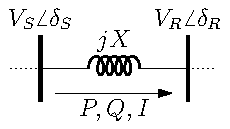
\includegraphics[width=.75\linewidth]{../../models/2bus/2bus}
\begin{align}
P &= \dfrac{V_R V_S}{X} \sin(\delta_S - \delta_R)\\
Q &= \dfrac{V_R}{X} \left(V_S\cos(\delta_S - \delta_R)-V_R\right)\\
I &= \dfrac{\abs{P + jQ}}{V_R\sqrt{3}}
\end{align}
(Plots on reverse)
		\item Generic Machine and Governors added and tested.
		\item dyd Parser updated to include MW capacity and percentages.
		\item WECC simulation works - takes 6 minutes for 30 second sim time. Generic governors used, islanded objects ignored, tap changers, SVD, and phase shifters enabled, PSLF exponential load changes handled.
	%	\item More \verb|matplotlib| plot functions created.

		\item GitHub updated:\\
		\verb|https://github.com/thadhaines/|
		
	\end{enumerate}
\paragraph{Current Tasks:}
	\begin{enumerate}
		\itemsep0em 
		\item Solidify test cases for validation
		\item `Interesting' Case generation
\subitem Large gov Deadband, fast AGC
\subitem Normal Deadband, adequate AGC (as per FERC requirements)
\subitem Various numbers of BA's 
		\item Continue to refine BA ACE actions.
\subitem Differentiate between reported ACE and distributed ACE
\subitem Enable FERC requirement checks
		\item Update Code flowchart% to aid in further development.
		\item Thesis work 
		%\item Keep Goals and Requests in mind.
		
		%\subitem A FlowtabrDAO exists that can find flow between busses. A way to initialize bus connections between areas has yet to be devised.

	\end{enumerate}

\vfill\null
\columnbreak

	\paragraph{Current Questions:}
	\begin{enumerate}
\itemsep0em 
	\item Progress on case data?
	\item VAR calculation - Real power and AMPS match, Reactive power off (see reverse)
	\end{enumerate}
	



% Common 2nd col removed 

\paragraph{Future Tasks:} %(Little to No Progress since last time / Things coming down the pipe)
	\begin{enumerate}
		
		\item Add import mirror / bypass mirror init sequence option to prevent repeated mirror creations.

		\item Bring wind into simulation \\ (ramp ungoverned generators?)


		
	\end{enumerate}
\paragraph{Future Work: (not by me)}
\begin{itemize}
\item Find best/correct way to trip gens in PSLF from python.
\item Account for different types of loads better. (exponential load model) % read from dyd
\item Work to incorporate Matt's \emph{Suggested Use Cases} into simulation.
		\begin{itemize}
		\item Add Shunt Group Agent
		\item Work to Define Definite Time Controller user input
		\end{itemize} 


		\item Investigate ULTC action.

		\item Create an agent for every object: \\ ULTC, SVD, Transformer, \ldots

		\item Move away from reliance on GE
		
\end{itemize}

\paragraph{Matt Requests:}
\begin{enumerate}
		\item Enable multiple dyd files to overwrite / replace previously defined agents/parameters
		\item Allow for variable time steps.
\end{enumerate}

\vfill\null
\end{multicols}

\pagebreak

\newcommand{\caseName}{SixMachineRamp1}
\begin{landscape}

\includegraphics[width=.33\linewidth,height=.33\textheight]{figures/\caseName Pbr1}%
\includegraphics[width=.33\linewidth,height=.33\textheight]{figures/\caseName Pbr2}%
\includegraphics[width=.33\linewidth,height=.33\textheight]{figures/\caseName Pbr3}

\includegraphics[width=.33\linewidth,height=.33\textheight]{figures/\caseName Qbr1}%
\includegraphics[width=.33\linewidth,height=.33\textheight]{figures/\caseName Qbr2}%
\includegraphics[width=.33\linewidth,height=.33\textheight]{figures/\caseName Qbr3}

\includegraphics[width=.33\linewidth,height=.33\textheight]{figures/\caseName Amp1}%
\includegraphics[width=.33\linewidth,height=.33\textheight]{figures/\caseName Amp2}%
\includegraphics[width=.33\linewidth,height=.33\textheight]{figures/\caseName Amp3}

\end{landscape}
\pagebreak

\textbf{Parsing Results from 2018 WECC case:}
Note: Dyd contains model information for objects no longer present in .sav - therefore, below values are only a 'ballpark' estimate of what actual model contains.

% Testing of external table build for \input later
\begin{table}[!ht]
	\centering
	\begin{tabular}{@{} C{2cm} 
	S[table-format=4.2,round-mode=places, round-precision=2,] 
	S[table-format=6.2,round-mode=places, round-precision=2] 
	S[table-format=3.2,round-mode=places, round-precision=2]
 	S[table-format=3.2,round-mode=places, round-precision=2] @{}} 	
		\toprule % @ signs to remove extra L R space
		\footnotesize % this will affect the table font (makse it 10pt)
		\raggedright % for non justified table text
Model Name & 	 \text{Occurrences} & 	 \text{MV Rating} & 		\text{\% Of Models}	&	\text{\% Of Capacity}	\\ \midrule
genrou & 	1823.000 & 	203122.050 & 	43.046 & 	54.651 \\
gentpj & 	1681.000 & 	117049.602 & 	39.693 & 	31.493 \\
gentpf & 	587.000 & 	34533.841 & 	13.861 & 	9.292 \\
gencc & 	48.000 & 	9790.800 & 	1.133 & 	2.634 \\
gewtg & 	52.000 & 	5528.296 & 	1.228 & 	1.487 \\
genwri & 	7.000 & 	839.210 & 	0.165 & 	0.226 \\
motor1 & 	37.000 & 	805.460 & 	0.874 & 	0.217 \\\midrule
TOTAL & 	4235.000 & 	371669.259 & 	100.000 & 	100.000 \\
		\bottomrule
	\end{tabular}
	\caption{Machine parsing results.}
	\label{tab: dydParse Machines }
\end{table}
% Testing of external table build for \input later
\begin{table}[!ht]
	\centering
	\begin{tabular}{@{} C{2cm} 
	S[table-format=4.2,round-mode=places, round-precision=2,] 
	S[table-format=6.2,round-mode=places, round-precision=2] 
	S[table-format=3.2,round-mode=places, round-precision=2]
 	S[table-format=3.2,round-mode=places, round-precision=2] @{}} 	
		\toprule % @ signs to remove extra L R space
		\footnotesize % this will affect the table font (makse it 10pt)
		\raggedright % for non justified table text
Model Name & 	 \text{Occurrences} & 	 \text{MW Cap} & 		\text{\% Of Models}	&	\text{\% Of Capacity}	\\ \midrule
ggov1 & 	1315.000 & 	77961.961 & 	46.060 & 	39.858 \\
ieeeg1 & 	300.000 & 	54452.110 & 	10.508 & 	27.838 \\
hyg3 & 	320.000 & 	18947.767 & 	11.208 & 	9.687 \\
hygov4 & 	167.000 & 	7614.401 & 	5.849 & 	3.893 \\
ieeeg3 & 	137.000 & 	7403.492 & 	4.799 & 	3.785 \\
hygovr & 	25.000 & 	6249.371 & 	0.876 & 	3.195 \\
ggov3 & 	30.000 & 	5358.317 & 	1.051 & 	2.739 \\
hygov & 	230.000 & 	5315.827 & 	8.056 & 	2.718 \\
pidgov & 	61.000 & 	3809.765 & 	2.137 & 	1.948 \\
wndtge & 	33.000 & 	3783.470 & 	1.156 & 	1.934 \\
gpwscc & 	62.000 & 	2398.050 & 	2.172 & 	1.226 \\
tgov1 & 	25.000 & 	1485.556 & 	0.876 & 	0.759 \\
g2wscc & 	21.000 & 	458.280 & 	0.736 & 	0.234 \\
gast & 	37.000 & 	330.680 & 	1.296 & 	0.169 \\
ccbt1 & 	3.000 & 	32.530 & 	0.105 & 	0.017 \\
wndtrb & 	1.000 & 	0.000 & 	0.035 & 	0.000 \\
lcfb1 & 	88.000 & 	0.000 & 	3.082 & 	0.000 \\ \midrule
TOTAL & 	2855.000 & 	195601.576 & 	100.000 & 	100.000 \\
		\bottomrule
	\end{tabular}
	\caption{Prime movers parsing results.}
	\label{tab: dydParse Prime Movers }
\end{table}
% Testing of external table build for \input later
\begin{table}[!ht]
	\centering
	\begin{tabular}{@{} C{2cm} 
	S[table-format=4.2,round-mode=places, round-precision=2,] 
	S[table-format=6.2,round-mode=places, round-precision=2] 
	S[table-format=3.2,round-mode=places, round-precision=2]
 	S[table-format=3.2,round-mode=places, round-precision=2] @{}} 	
		\toprule % @ signs to remove extra L R space
		\footnotesize % this will affect the table font (makse it 10pt)
		\raggedright % for non justified table text
Model Name & 	 \text{Occurrences} & 	 \text{MW Cap} & 		\text{\% Of Models}	&	\text{\% Of Capacity}	\\ \midrule
regc\_a & 	286.000 & 	18461.697 & 	19.536 & 	40.287 \\
wt4g & 	131.000 & 	8995.084 & 	8.948 & 	19.629 \\
wt3g & 	112.000 & 	7633.716 & 	7.650 & 	16.658 \\
wt3e & 	106.000 & 	4882.038 & 	7.240 & 	10.654 \\
wt2g & 	21.000 & 	1841.236 & 	1.434 & 	4.018 \\
wt2t & 	19.000 & 	1224.900 & 	1.298 & 	2.673 \\
wt1g & 	21.000 & 	1188.370 & 	1.434 & 	2.593 \\
wt1t & 	21.000 & 	885.990 & 	1.434 & 	1.933 \\
wt3t & 	106.000 & 	712.280 & 	7.240 & 	1.554 \\
wtgt\_a & 	35.000 & 	0.000 & 	2.391 & 	0.000 \\
wtgq\_a & 	29.000 & 	0.000 & 	1.981 & 	0.000 \\
wtgp\_a & 	29.000 & 	0.000 & 	1.981 & 	0.000 \\
wtga\_a & 	28.000 & 	0.000 & 	1.913 & 	0.000 \\
wt4t & 	72.000 & 	0.000 & 	4.918 & 	0.000 \\
%wt4e & 	128.000 & 	0.000 & 	8.743 & 	0.000 \\
wt3p & 	67.000 & 	0.000 & 	4.577 & 	0.000 \\
wt2p & 	16.000 & 	0.000 & 	1.093 & 	0.000 \\
wt2e & 	19.000 & 	0.000 & 	1.298 & 	0.000 \\
wt1p & 	16.000 & 	0.000 & 	1.093 & 	0.000 \\
repc\_a & 	143.000 & 	0.000 & 	9.768 & 	0.000 \\
reec\_a & 	44.000 & 	0.000 & 	3.005 & 	0.000 \\
exwtg1 & 	5.000 & 	0.000 & 	0.342 & 	0.000 \\
ewtgfc & 	10.000 & 	0.000 & 	0.683 & 	0.000 \\ \midrule
TOTAL & 	1464.000 & 	45825.311 & 	100.000 & 	100.000 \\
		\bottomrule
	\end{tabular}
	\caption{Wind turbine parsing results.}
	\label{tab: dydParse wind turbines }
\end{table}

%\paragraph{'Soft Goals':}
%	\begin{enumerate}
%	\item Write Thesis 2020
%	\end{enumerate}
		

\end{document}